
\documentclass[dvipdfmx,autodetect-engine]{jreport}
\usepackage[top=30truemm,bottom=30truemm,left=25truemm,right=25truemm]{geometry}
\usepackage[dvipdfmx]{graphicx}
\usepackage{float}
\usepackage{natbib}
\usepackage{subfig}

\title{タイコグラフィによる回転体X線結像ミラーのキャラクタリゼーション}
\author{dieu.detruit }
\date{December 2020}

\begin{document}

\begin{center}
\thispagestyle{empty}
{\LARGE 令和2年度 卒業論文}\\
\begin{figure}[H]
    \centering
    
\includegraphics[scale=0.4]{images/utility/utlogo.jpg}
\end{figure}
\vspace*{2.5cm}
{\Huge タイコグラフィ法による}\\
\vspace*{0.5cm}
{\Huge 回転体X線結像ミラーの}\\
\vspace*{0.5cm}
{\Huge キャラクタリゼーション}\\
\vspace*{1.5cm}
{\huge Characterization of Rotation X-ray Imaging Mirror}\\
\vspace*{0.5cm}
{\huge Using Ptychographical Method}\\
\vspace*{3.5cm}
{\LARGE 指導教員 三村 秀和 准教授}\\
\vspace*{1.0cm}
{\Large 東京大学 工学部 精密工学科}\\
{\Large 03-190395}\\
\vspace*{1.0cm}
{\LARGE 渡辺 貴史}
\end{center}

\newpage
\tableofcontents

\newpage
\chapter{序論}
\section{研究の意義・背景}
通常、我々が天体を観測するとき、可視光を通してその形状や特徴を観察する。一方で、天文学では熱や電磁波、放射線といった可視光以外の媒体を通じて様々な現象が明らかにされてきた。中でも、電磁波の一種であるX線を観測することは、天文学において非常に有用である。2018年に打ち上げられたFOXSI3では太陽コロナのX線写真を撮影することに成功し、その物理をより明らかにするに至った。図\ref{fig:foxsi-fullsun-image}はその撮影像の1枚である。太陽コロナを満たす高温のプラズマから放射される電磁波はX線の領域であり、これを撮影することは長年の課題であった。X線は大気により吸収されやすいという特徴を持つため、宇宙に打ち上げられたロケットから観察する必要がある。またこの上でさらに時間分解能と空間分解能の両方を十分に確保して撮影しなければならず、非常に難しい問題であった。これを可能にした一つの要素として、Wolter型ミラーが挙げられる。

\begin{figure}[h!]
\centering
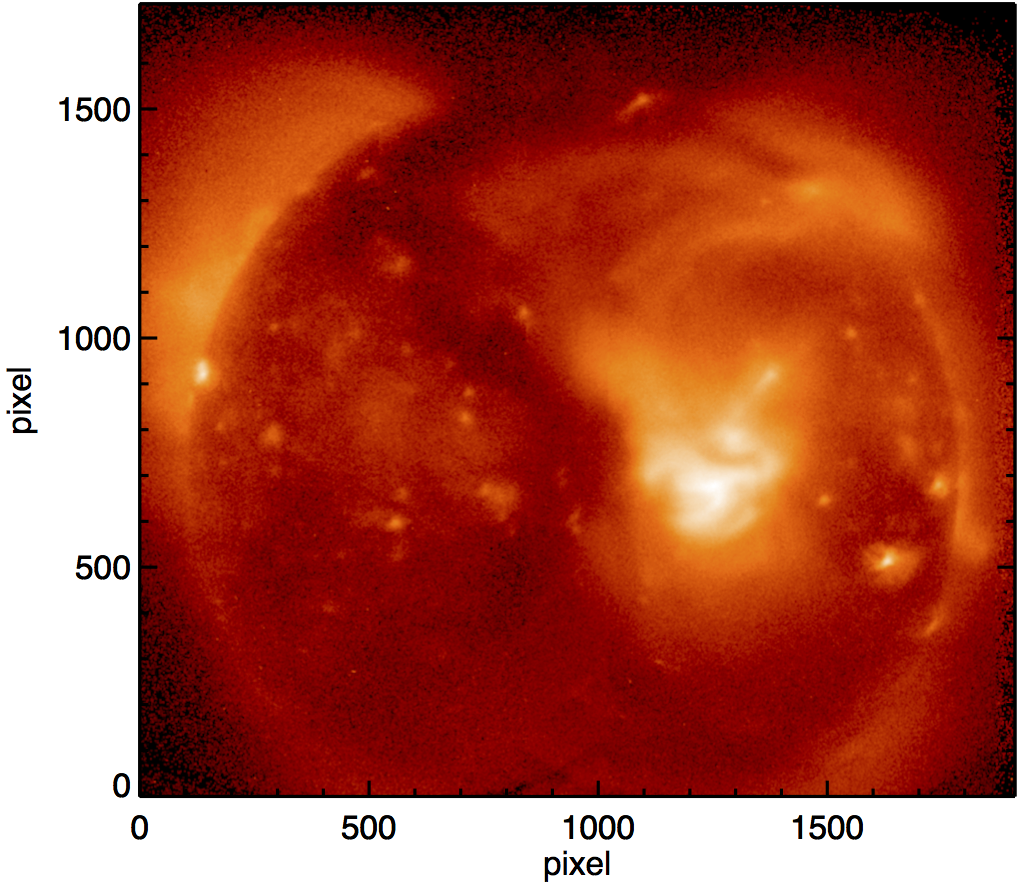
\includegraphics[scale=1.0]{images/foxsi/foxsi3-full-sun.png}
\caption{FOXSI-3 PhoEnIx full Sun Soft X-ray image}
\label{fig:foxsi-fullsun-image}
\end{figure}

\section{Wolterミラー}
光を一点に集光するための素子として、屈折を利用するレンズ、反射を利用したミラー、回折を利用したフレネルゾーンプレートなどが有名である。


\section{従来的な直接計測法}

\newpage
\chapter{Wolterミラーの誤差応答シミュレーション}

この節では、シミュレーションの方法について述べる。


\newpage
\section{諸言}
Wolterミラーを光学系に組み込んで利用する際、大きく分けて2つの誤差によってその理想の集光・結像が損なわれる。ひとつは設計曲面と実際に加工されたミラー表面の形状の誤差、もうひとつはミラー設置時の位置・姿勢の誤差である。
これらを与えたとき集光点の様子がどのようになるか、また集光点の変化として許容できる誤差の範囲はどれほどなのかを見積もることは、Wolterミラー評価の重要な軸となる。6章では、加工されたミラーに対して測定実験を行い、本章で計算した許容誤差との比較・検討を行う。

\section{誤差の評価と許容される誤差}
結像または集光を行う光学系の是非が、集光面での波面が理想からどれだけ離れているかということで評価されるということを先に述べた。では、理想の集光波面との差異を定量的に評価するためには、具体的な評価軸が必要である。そこで主に用いられるのが、Strehl比、HPD、FWHMの3つの特徴量である。

\subsection{Strehl比}
主に集光光学系の文脈において、理想の集光状態を回折限界集光」と呼ぶ。十分にこの状態に近いと言えるための1つの指標として用いられるのが、Strehl比である。Strehl比とは、実際の集光波面における最大値と回折限界時の集光波面における最大値の比である。つまり、振幅を$I(\mathbf{r})$として

\[
r_{\mathrm{Strehl}} = \frac{ \max{\sqrt{I(\mathbf{r})} } }{ \max{ \sqrt{I_{\mathrm{ideal}}( \mathbf{r} )} } }
\]

と定義される。図\ref{fig:strehl_explanation}にその模式的なグラフを示す。このStrehl比が0.8以上であるとき、その系は回折限界集光をしている、としたのがMareshal基準である\citep{BornWolf:1999:Book}。この0.8という値には体系的な根拠はなく、解析・実験における経験的な指標として扱われている。本論文では、この慣例を踏襲し、0.8を閾値としてStrehl比を評価する。

\begin{figure}[h!]
\centering
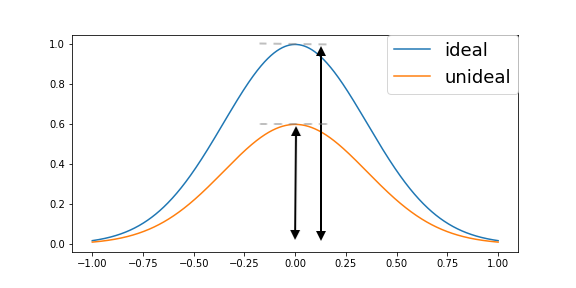
\includegraphics[scale=0.6]{images/error_simulation/explanation/strehl.png}
\caption{Strehl比計算の模式図}
\label{fig:strehl_explanation}
\end{figure}

\subsection{HPD(Half Power Diameter)}
Strehl比による比較検討では「回折限界集光をしていると言えるか」に主眼を置いているが、天文用Wolterミラーのように達成すべき角度分解能が決まっている場合では直接その分解能要求を満たしているかどうかを判定するのが実用的である。分解能を決定するのは、焦点面におけるビームの集光サイズであり、これは大きく2つの定義によって議論される。その一つが、Half Power Diameter(半値幅、HPD)である。HPDの定義は「焦点面上の全強度の50\%の強度を含む円の直径」である。つまり、
\[
    \sum_{d\leq d_{\mathrm{HPD}}} \sqrt{ I(\mathbf{r}) } = \frac{1}{2} \sum \sqrt{ I(\mathbf{r}) }
\]
を満たすような直径$d_{\mathrm{HPD}}$として定義される。図\ref{fig:hpd_explanation}にその例を示す。この赤円の内側の強度総和値は、全体の強度総和値の半分になっている。

\begin{figure}[h!]
\centering
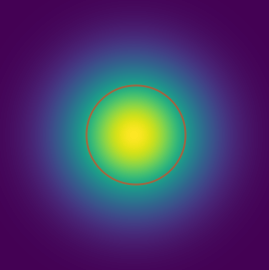
\includegraphics[scale=0.6]{images/error_simulation/explanation/HPD.png}
\caption{HPDの例}
\label{fig:hpd_explanation}
\end{figure}

\subsection{FWHM(Full Width Half Maximum)}
HPDに並んでビーム集光サイズの評価として用いられるのが、FWHM(Full Width Half Maximum)である。こちらは焦点面を集光点を通る直線によって切断したプロファイルに対して、「焦点面における最大値の半分の値を取る2点の距離」と定められる。図\ref{fig:fwhm_explanation_profile}は1つのプロファイルに対するFWHMの例である。切断する直線には任意性があるため、通常は図\ref{fig:fwhm_explanation}のように水平方向と鉛直方向の切断しこれを評価する。

\begin{figure}[h!]
\centering
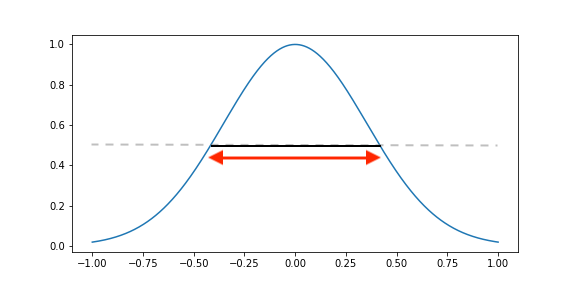
\includegraphics[scale=0.6]{images/error_simulation/explanation/FWHM.png}
\caption{FWHMの例}
\label{fig:fwhm_explanation_profile}
\end{figure}

\begin{figure}[h!]
\centering

\subfloat[horizontal]{
    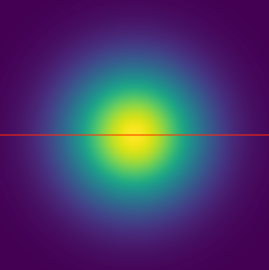
\includegraphics[scale=0.6]{images/error_simulation/explanation/FWHM_horizontal.png}
    \label{fig:fwhm_explanation_horizontal}
}
\subfloat[vertical]{
    \centering
    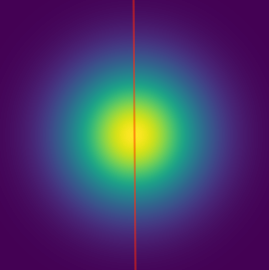
\includegraphics[scale=0.6]{images/error_simulation/explanation/FWHM_vertical.png}
    \label{fig:fwhm_explanation_vertical}
}
\caption[]{切断の例 水平:\subref{fig:fwhm_explanation_horizontal}, 鉛直:\subref{fig:fwhm_explanation_vertical}}
\label{fig:fwhm_explanation}
\end{figure}

\section{シミュレーションの方法}
のこの節では、シミュレーションの方法について述べる。

\section{計算条件}
6章で実際に利用する測定対象のミラーについて、誤差応答のシミュレーションを行う。以下にその設計パラメータを示す。




\section{直径誤差}

\section{扁平誤差}

\section{周方向形状誤差}

\section{長手方向形状誤差}

\section{設置角度誤差}

\section{設置位置誤差}

\newpage
\chapter{Wolterミラー評価実験の手法に関する検討}

\newpage
\section{位相回復法の概要}

\section{タイコグラフィ法の概要}
2章でも述べた通り、波面計測は波動光学に基づいており、X線の伝播は複素波動場として与えられる。一方で、CCDカメラなどの撮像素子で得られるのはその振幅の2乗、つまりエネルギーの情報のみである。

\section{焦点面走査による冗長性}
前節で述べた方法について、用いるオブジェクトには大きく分けて2種類ある。1つは透過関数として表現される

\section{疎条件の利用}
輪帯状でかつ細い波面を回復するという問題において、回復領域の面積は下流端開口面の伝播領域全体に対して非常に小さい。このことは、主にCDI(コヒーレント回折イメージング)の文脈で利用される、期待される波面領域以外の場所で振幅が0であるという情報を使い位相を回復する方法が有効であることを示す。位相回復とは未知数に対して十分に冗長な数の方程式が与えられることであったのだから、未知数が激減することは回を求める上で非常に有用である。
CDIで広く使われているアルゴリズムの1つが、HIO(Hybrid Iterative Engine)であり、この系にも適用することが可能である。

\section{ディテクター走査による冗長性}

\section{下流端開口走査による冗長性}

\subsection{対称性}

\newpage
\chapter{レンズによる提案手法の検討}

\newpage

\section{実験の構成}
実験装置の概要を以下に示す。
平行光に対して輪帯状の開口を入れることで、擬似的に輪帯開口の集光光学系を再現する。
輪帯開口の設計

\section{実験の構成}
実験装置の概要を以下に示す。


\newpage
\chapter{結論}
``I always thought something was fundamentally wrong with the universe'' \citep{adams1995hitchhiker}

\newpage
\chapter{謝辞}
ありがとうそしてありがとう

\bibliographystyle{plain}
\bibliography{references}

\end{document}

